\begin{frame}
	\myheading{Module 13.5 : Guided Backpropagation}
\end{frame}

%%%%%%%%%%%%%%%%%%%%%%%%%%%%%%%%%%%%%%%%%%%%%%%%%%%%%%%%%%%%%%%%%%%%%%%%%%%%%%%%%%%%%%%%%
			
\begin{frame}
	\begin{columns}
		
		
		\column{0.5\textwidth}
		\begin{overlayarea}{\textwidth}{\textheight}
		
		\begin{tikzpicture}
	\only<1>{\node at (+3.5,-0.0) (figa) { 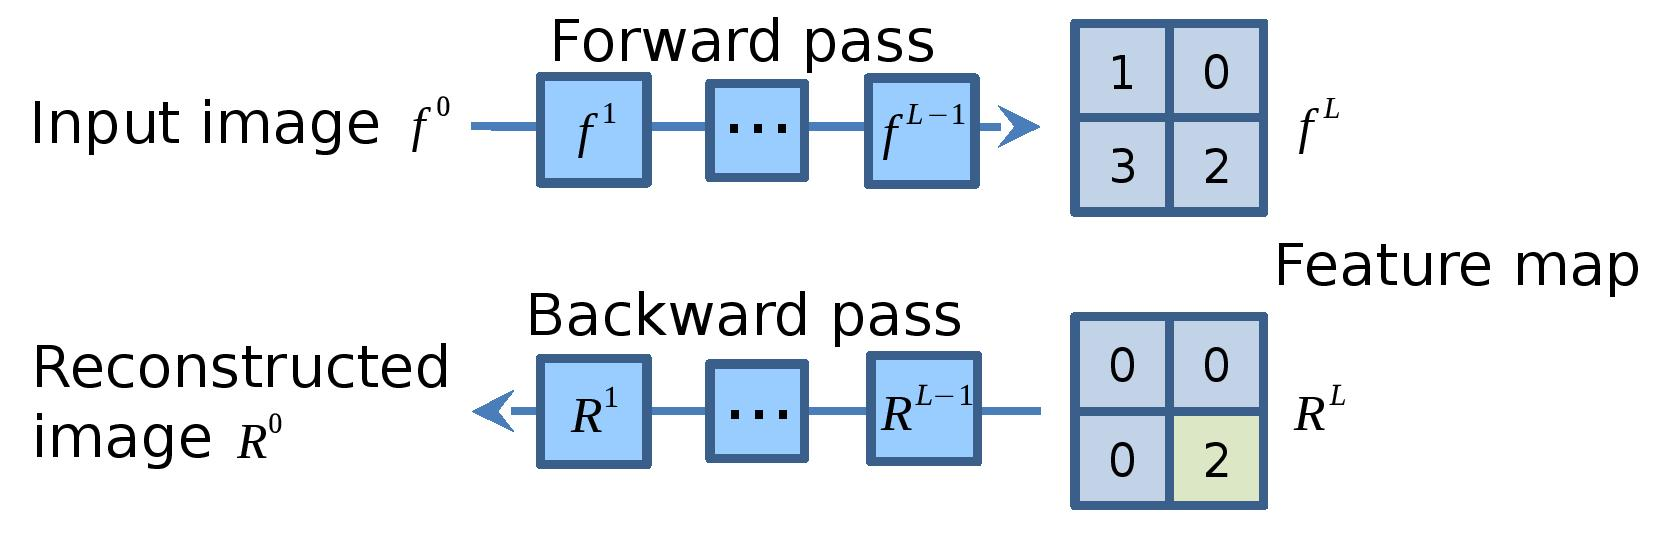
\includegraphics[scale=0.4,trim={0cm 2.5cm 0cm 0cm},clip=true]{images/3_1_1.jpg}};}
	\only<2->{\node at (+3.5,-0.0) (figb) { 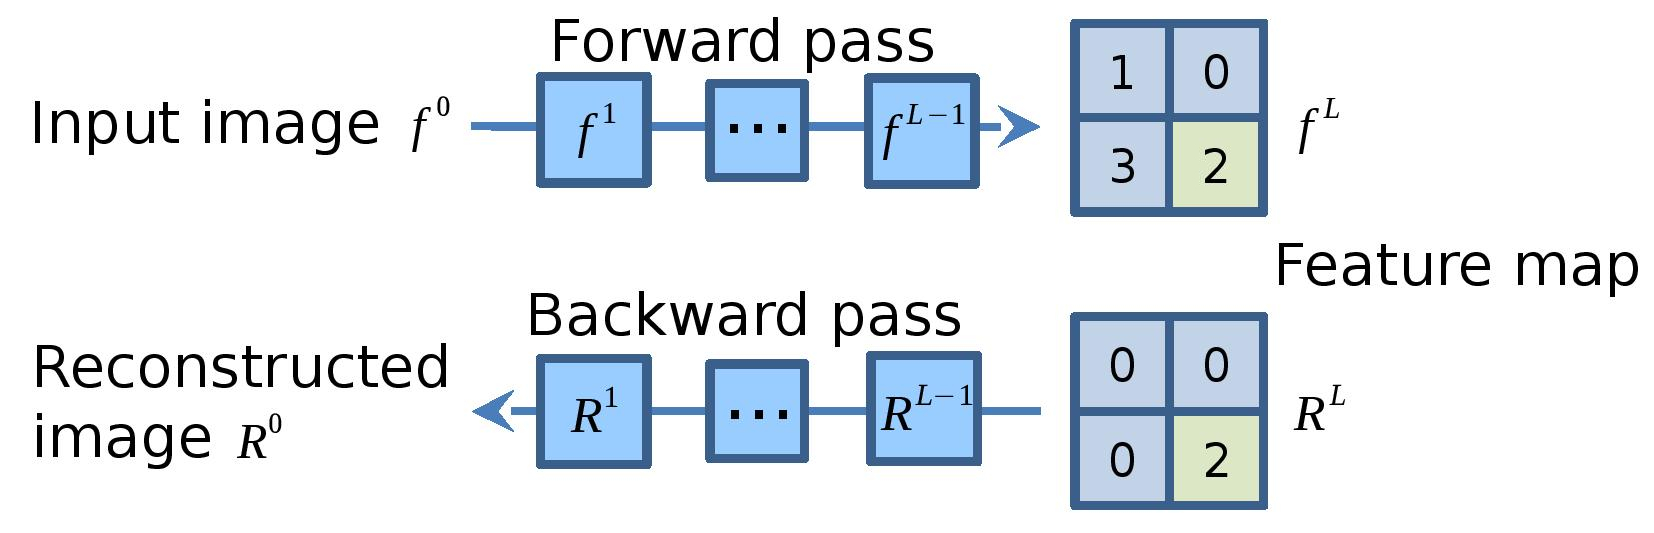
\includegraphics[scale=0.4,trim={0cm 2.5cm 0cm 0cm},clip=true]{images/3_1_2.jpg}};}
	\onslide<4->{\node at (5.1,-1) (figc) { 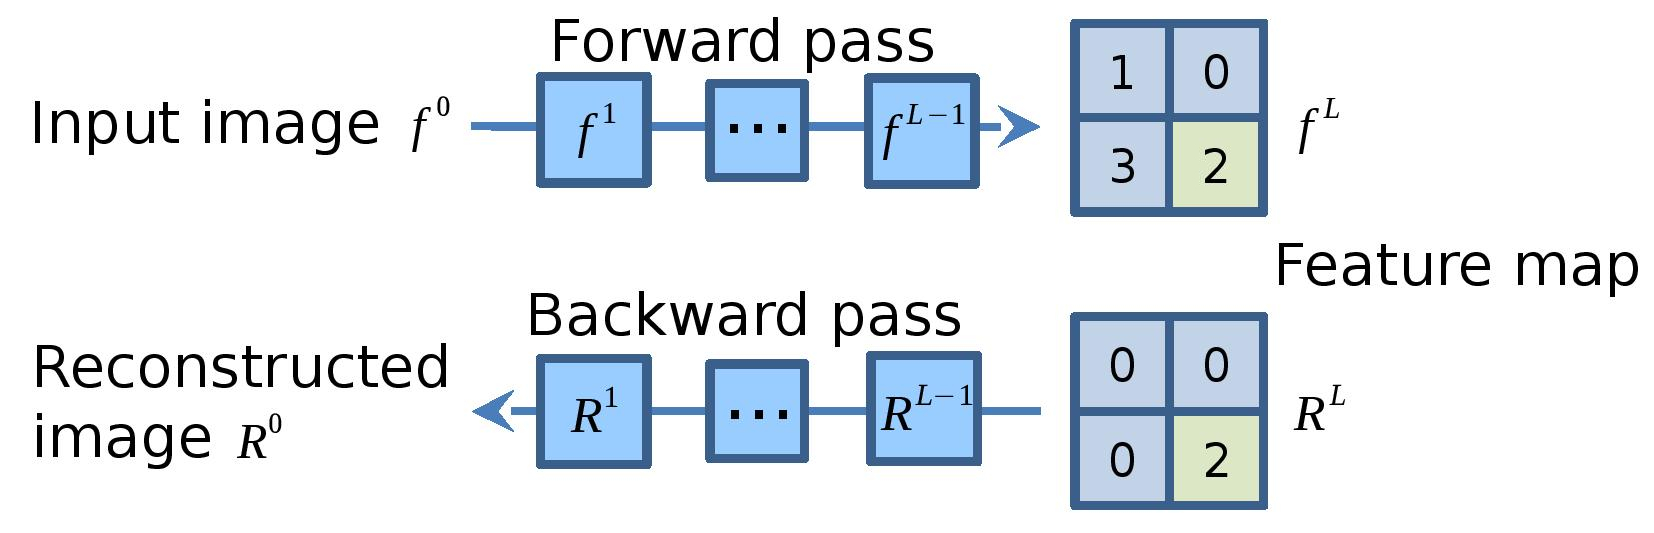
\includegraphics[scale=0.4,trim={9cm 0cm 1cm 2.5cm},clip=true]{images/3_1_2.jpg}};}
\end{tikzpicture}
		\end{overlayarea}
		\column{0.5\textwidth}
		\begin{overlayarea}{\textwidth}{\textheight}
			\begin{itemize}
				\justifying
				\onslide<1->{\item We feed an input to the CNN and do a forward pass}
				\onslide<2->{\item We consider one neuron in some feature map at some layer}
				\onslide<3->{\item We are interested in finding the influence of the input on this neuron}
				\onslide<4->{\item We retain this neuron and set all other neurons in the layer to zero}
			\end{itemize}
			
		\end{overlayarea}
	\end{columns}
\end{frame}

%%%%%%%%%%%%%%%%%%%%%%%%%%%%%%%%%%%%%%%%%%%%%%%%%%%%%%%%%%%%%%%%%%%%%%%%%%%%%%%%%%%%%%%%%

\begin{frame}
	\begin{overlayarea}{\textwidth}{\textheight}
		\begin{columns}
			\column{0.5\textwidth}
			\begin{tikzpicture}
	\onslide<1->{\node at (1.0,0.0) (figa)  { 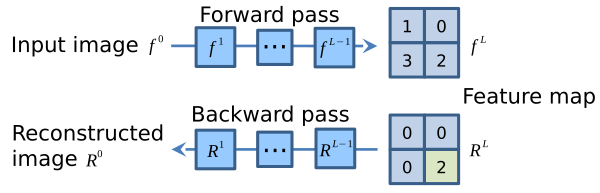
\includegraphics[scale=0.4]{images/3_2_1.jpg}};}
	\onslide<2->{\node at (0,-2) (figb)  { 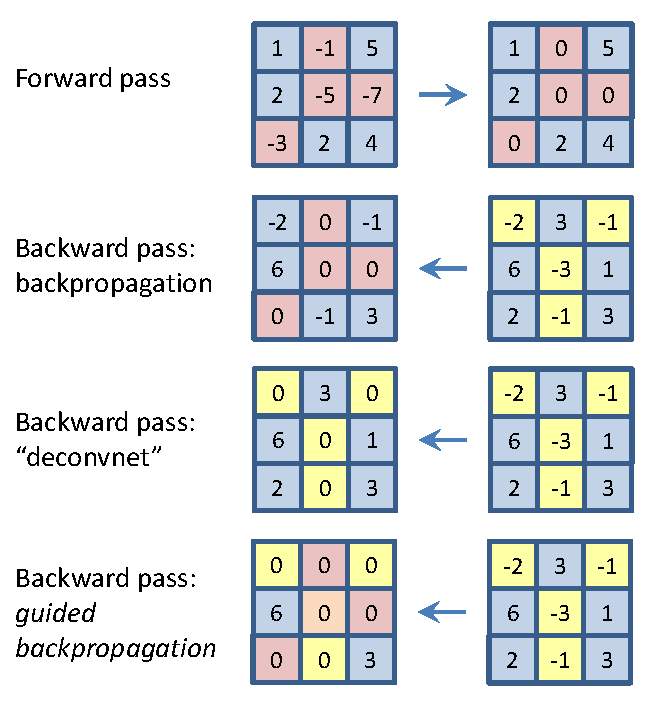
\includegraphics[scale=0.5,trim={0cm 9cm 0cm 0cm},clip=true]{images/3_2_2.pdf}};}
	\onslide<3->{\node at (0,-4) (figc)  { 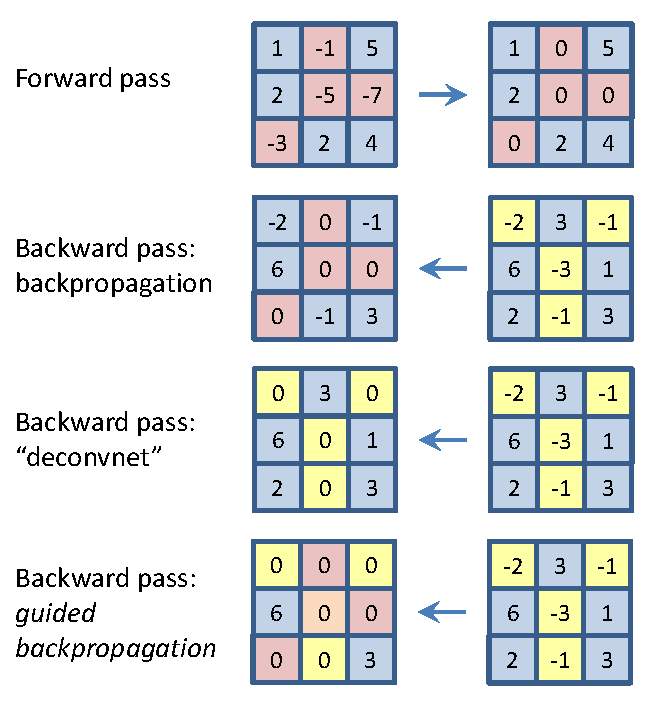
\includegraphics[scale=0.5,trim={0cm 6cm 0cm 3cm},clip=true]{images/3_2_2.pdf}};}
	\onslide<4->{\node at (0,-6) (figd)  { 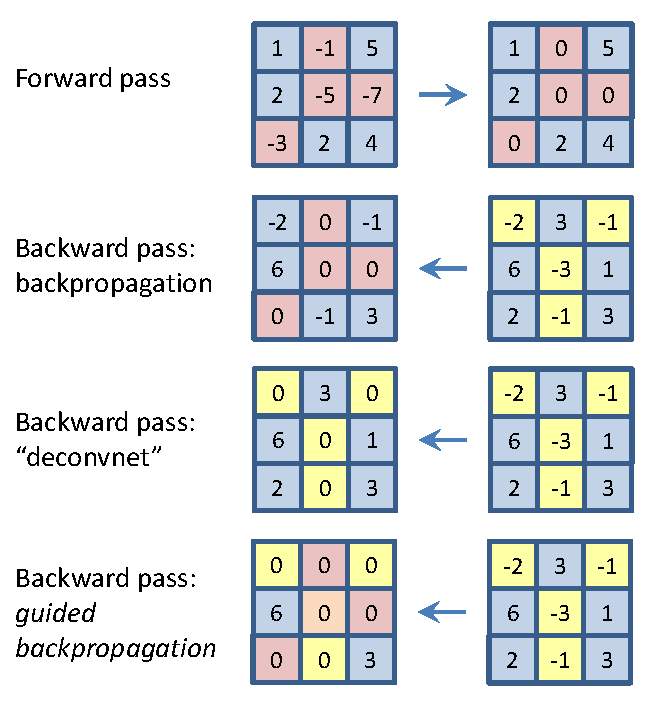
\includegraphics[scale=0.5,trim={0cm 0cm 0cm 9cm},clip=true]{images/3_2_2.pdf}};}
\end{tikzpicture}
				
			\column{0.5\textwidth}
			
			\begin{itemize}
				\justifying
				\onslide<1->{\item We now backpropogate all the way to the inputs}
				\onslide<2->{\item Recall that during forward pass relu activation allows only positive values to pass \& clamps $-ve$ values to zero}
				\onslide<3->{\item Similarly during backward pass no gradient passes through the dead relu neurons}
				\onslide<4->{\item In guided back propagation any -ve gradients flowing from the upper layer are also set to 0}
			\end{itemize}
					
		\end{columns}
	\end{overlayarea}
\end{frame}

%%%%%%%%%%%%%%%%%%%%%%%%%%%%%%%%%%%%%%%%%%%%%%%%%%%%%%%%%%%%%%%%%%%%%%%%%%%%%%%%%%%%%%%%%

\begin{frame}
	\begin{overlayarea}{\textwidth}{\textheight}
		\begin{columns}
			\column{0.5\textwidth}
			\begin{center}
				\begin{tikzpicture}
	\onslide<1->{\node at (4.0,-0.0) (figa)  { 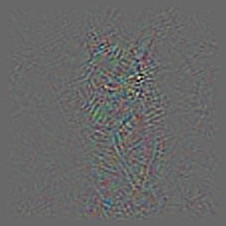
\includegraphics[scale=0.3]{images/2_4_1.png}};
		\node (texta) [below right = 1mm and -3mm of figa, anchor=east]{\tiny \textsf{Backpropagation}};}
	\onslide<2->{\node at (4,-3.5) (figb)  { 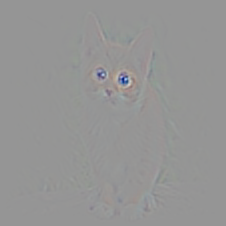
\includegraphics[scale=0.3]{images/2_4_2.png}};
		\node (textb) [below right = 1mm and 1mm of figb, anchor=east]{\tiny \textsf{Guided Backpropagation}};}
\end{tikzpicture}
			\end{center}
			
			\column{0.5\textwidth}
			
			\begin{itemize}
				\justifying
				\onslide<1->{\item \textbf{Intuition:} Neglect all the negative influences (gradients) and focus only on the positive influences (gradients)}				
				\onslide<2->{\item This gives a better picture of the true influence of the input}			
			\end{itemize}
					
		\end{columns}
	\end{overlayarea}
\end{frame}
